\documentclass[border=4pt]{standalone}
\usepackage{mathptmx}
\usepackage[T1]{fontenc}
\usepackage{tikz}
\usetikzlibrary{shapes.geometric,arrows.meta,positioning,fit,calc,backgrounds}
\begin{document}

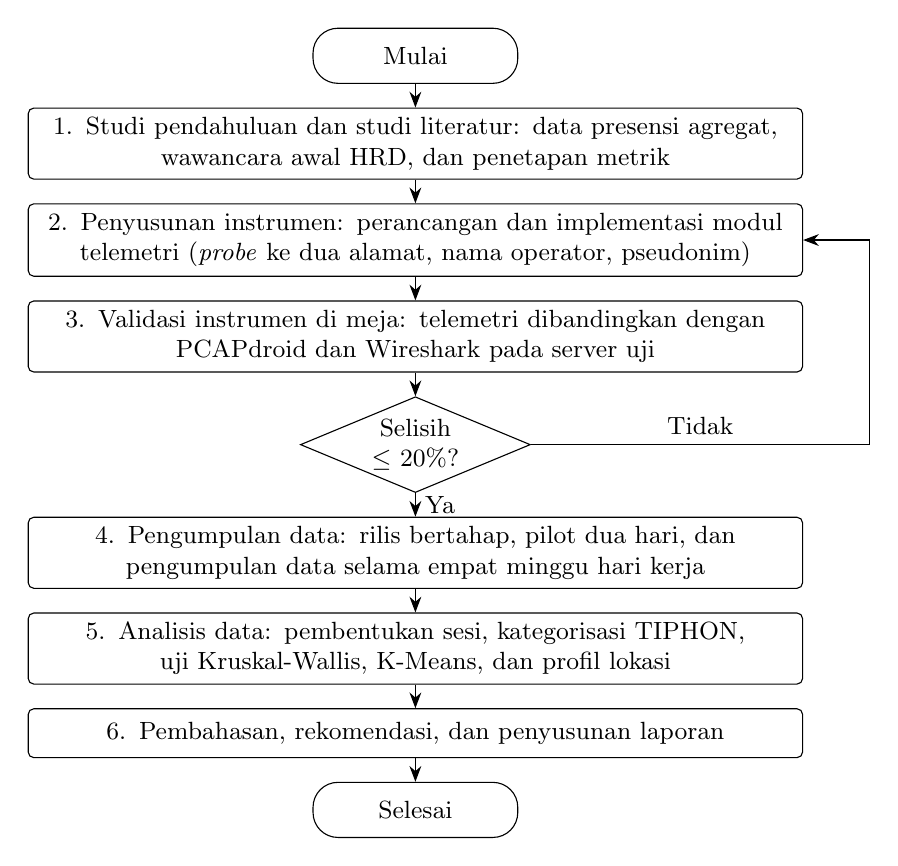
\begin{tikzpicture}[
    node distance=0.30cm,
    proses/.style={rectangle, draw, rounded corners=2pt, align=center, text width=9.6cm, minimum height=0.62cm, font=\small},
    batas/.style={rectangle, draw, rounded corners=9pt, align=center, minimum width=2.6cm, minimum height=0.7cm, font=\small},
    keputusan/.style={diamond, draw, aspect=2.4, align=center, inner sep=1pt, font=\small},
    panah/.style={-{Stealth[length=2mm]}}
]
\node[batas] (mulai) {Mulai};
\node[proses, below=of mulai] (s1) {1. Studi pendahuluan dan studi literatur: data presensi agregat,\\ wawancara awal HRD, dan penetapan metrik};
\node[proses, below=of s1] (s2) {2. Penyusunan instrumen: perancangan dan implementasi modul\\ telemetri (\textit{probe} ke dua alamat, nama operator, pseudonim)};
\node[proses, below=of s2] (s3) {3. Validasi instrumen di meja: telemetri dibandingkan dengan\\ PCAPdroid dan Wireshark pada server uji};
\node[keputusan, below=of s3] (k) {Selisih\\$\le$ 20\%?};
\node[proses, below=of k] (s4) {4. Pengumpulan data: rilis bertahap, pilot dua hari, dan\\ pengumpulan data selama empat minggu hari kerja};
\node[proses, below=of s4] (s5) {5. Analisis data: pembentukan sesi, kategorisasi TIPHON,\\ uji Kruskal-Wallis, K-Means, dan profil lokasi};
\node[proses, below=of s5] (s6) {6. Pembahasan, rekomendasi, dan penyusunan laporan};
\node[batas, below=of s6] (selesai) {Selesai};
\draw[panah] (mulai) -- (s1);
\draw[panah] (s1) -- (s2);
\draw[panah] (s2) -- (s3);
\draw[panah] (s3) -- (k);
\draw[panah] (k) -- node[right, font=\small] {Ya} (s4);
\draw[panah] (s4) -- (s5);
\draw[panah] (s5) -- (s6);
\draw[panah] (s6) -- (selesai);
\draw[panah] (k.east) -- node[above, font=\small] {Tidak} ++(4.3,0) |- (s2.east);
\end{tikzpicture}
\end{document}
